% Created 2016-02-18 tor 20:27
% Indented LaTeX compiler: pdflatex
\documentclass[12pt,twoside]{article}
\usepackage[utf8]{inputenc}
\usepackage[T1]{fontenc}
\usepackage{graphicx}
\usepackage{grffile}
\usepackage{longtable}
\usepackage{wrapfig}
\usepackage{rotating}
\usepackage[normalem]{ulem}
\usepackage{amsmath}
\usepackage{textcomp}
\usepackage{amssymb}
\usepackage{capt-of}
\usepackage{hyperref}
\usepackage{tabularx}
\usepackage{minted}
\usepackage[paper=a4paper,dvips,top=1.5cm,left=1.5cm,right=1.5cm, foot=1cm,bottom=1.5cm]{geometry}
\renewcommand{\rmdefault}{ptm}
\usepackage[scaled=.90]{helvet}
\usepackage{courier}
\usepackage{bookmark}
\usepackage{fancyhdr}
\pagestyle{fancy}
\usepackage[dvipsnames*,svgnames]{xcolor}
\usepackage{tikz}
\usetikzlibrary{arrows,decorations.pathmorphing,backgrounds,fit,positioning,calc,shapes}
\usepackage[utf8]{inputenc}
\usepackage[swedish, english]{babel}
\usepackage{rotating}
\usepackage{array}
\usepackage{graphicx}
\usepackage{float}
\usepackage{color}
\usepackage{mdwlist}
\usepackage{setspace}
\usepackage{listings}
\usepackage{bytefield}
\usepackage{tabularx}
\usepackage{multirow}
\usepackage{algorithm}
\usepackage{algpseudocode}
\usepackage{dcolumn}
\usepackage{url}
\usepackage[perpage,para,symbol]{footmisc}
\usepackage[all]{hypcap}
\definecolor{darkblue}{rgb}{0.0,0.0,0.3} %% define a color called darkblue
\definecolor{darkred}{rgb}{0.4,0.0,0.0}
\definecolor{red}{rgb}{0.7,0.0,0.0}
\definecolor{lightgrey}{rgb}{0.8,0.8,0.8}
\definecolor{grey}{rgb}{0.6,0.6,0.6}
\definecolor{darkgrey}{rgb}{0.4,0.4,0.4}
\hyphenpenalty=15000
\tolerance=1000
\newcommand{\rr}{\raggedright}
\newcommand{\rl}{\raggedleft}
\newcommand{\tn}{\tabularnewline}
\newcommand{\colorbitbox}[3]{%
\rlap{\bitbox{#2}{\color{#1}\rule{\width}{\height}}}\bitbox{#2}{#3}}
\newcommand{\red}{\color{red}}
\makeatletter
\renewcommand\paragraph{\@startsection{paragraph}{4}{\z@}{-3.25ex\@plus -1ex \@minus -.2ex}{1.5ex \@plus .2ex} {\normalfont\normalsize\bfseries}}
\makeatother
\makeatletter
\renewcommand\subparagraph{\@startsection{subparagraph}{5}{\z@}{-3.25ex\@plus -1ex \@minus -.2ex}{1.5ex \@plus .2ex} {\normalfont\normalsize\bfseries}}
\makeatother
\setcounter{tocdepth}{3}
\setcounter{secnumdepth}{5}
\renewcommand{\headrulewidth}{0pt}
\lhead{K.Sotiropoulos: Master's Thesis}
\chead{Project Plan version 1}
\rhead{\date{\today}}
\makeatletter
\let\ps@plain\ps@fancy
\makeatother
\setlength{\headheight}{15pt}
\date{}
\title{Project Title: Parallel Simulation of SystemC Loosely-Timed Transaction Level Models}
\hypersetup{
 pdfauthor={Konstantinos Sotiropoulos},
 pdftitle={Project Title: Parallel Simulation of SystemC Loosely-Timed Transaction Level Models},
 pdfkeywords={},
 pdfsubject={},
 pdfcreator={Emacs 24.3.1 (Org mode 8.3.2)}, 
 pdflang={English}}
\begin{document}

\author{
        \textsc{Konstantinos Sotiropoulos}
        \mbox{}\\
        \normalsize
            \texttt{konstantinos.sotiropoulos}
        \normalsize
            \texttt{@intel.com}
}

\date{\today}

\maketitle

\tableofcontents

\clearpage

\section{Acronyms}
\label{sec:orgheadline1}
\begin{center}
\begin{tabular}{ll}
\textbf{DE}: & Discrete Event\\
\textbf{DES}: & Discrete Event Simulator/Simulation\\
\textbf{DMI}: & Direct Memory Interface\\
\textbf{ESL}: & Electronic System-Level Design\\
\textbf{HPC}: & High Performance Computing\\
\textbf{MoC}: & Model of Computation\\
\textbf{MPSoC}: & Multicore System on Chips\\
\textbf{OoO}: & Out-of-Order\\
\textbf{PDES}: & Parallel Discrete Event Simulation\\
\textbf{SLDL}: & System-Level Design Language\\
\textbf{SMP}: & Symmetric Multiprocessing\\
\textbf{SoC}: & System on Chip\\
\textbf{SR}: & Synchronous Reactive\\
\textbf{TLM}: & Transaction Level Modeling\\
\textbf{CMB}: & Chandy/Misra/Bryant algorithm\\
\end{tabular}
\end{center}
\clearpage


\section{Organization}
\label{sec:orgheadline2}
This is a Master's Thesis project that will be carried out in Intel Sweden AB and is supervised by KTH's ICT department.
Mr. Bjorn Runaker (\texttt{bjorn.runaker@intel.com}) is the project's supervisor from the company's side, 
while professor \href{https://people.kth.se/~ingo/}{Ingo Sanders} (\texttt{ingo@kth.se}) and PhD student \href{http://people.kth.se/~ugeorge/}{George Ungureanu} (\texttt{ugeorge@kth.se})are the examiner and supervisor from KTH. 
The project begun on 2016-01-16 and will finish on 2016-06-30, as dictated by the contract of employment that I, Konstantinos Sotiropoulos a Master's student at the Embedded Systems program, have signed with the company 
(document title: "Statement of Terms and Conditions of Fixed Term Employment"). 

The scope of this project has been and is being mutually determined by all parties. 
It is dialectically determined between the company's needs and the institute's research agenda.
As Master's Thesis project, it needs to expose a scientific ground on which the engineering effort shall be rooted.

All the necessary equipment (software and hardware) has been kindly provided by the company.
The exact legal context that will apply to any software produced as a result of this project is yet to be determined, 
but will conform to the general context dictated by the documents already signed (documents' titles:  "Statement of Terms and Conditions of Fixed Term Employment" and "Employee Agreement") .




\section{Background}
\label{sec:orgheadline8}
SystemC is considered to be a System-Level Design Language (SLDL), that is implemented as a C++ class library.
The language is maintained and promoted by Accellera (former Open SystemC Initiative OSCI) and has been standardized with the latest LRB being the IEEE 1666-2011 \cite{OpenSystemCInitiative2012}
The major advantage SystemC provides to the designer is that a component's functionality can be easily expressed in C/C++, the dominating languages for in systems programming (e.g. Operating System and Device Driver development).
As a result SystemC models are executable: the designer can directly simulate the behavior of a system modeled in SystemC.
The language has been demanded and supported by the semiconductor industry, in its collaborative effort to push Electronic Design Automation (EDA) into higher abstraction layers, thus giving birth to a trend
referred to as Electronic System-Level Design (ESLD).

The rest of this section is devoted into presenting the theoretical/scientific ground on which we will cultivate this project.
To avoid confusion by being precise, fundamental terms and concepts of computer science are being defined and redefined, even at the risk of being pedantic.  
Facing a labyrinth of abstraction layers, we will begin unraveling Ariadne's thread at the simple observation that SystemC is a System Level Design \textbf{Language}.

\subsection{Models of Computation}
\label{sec:orgheadline3}
A \textbf{language} is a set of symbols, rules for combining them (its syntax), and rules for interpreting combinations of symbols (its semantics). 
Two approaches to semantics have evolved: denotational and operational.
Operational semantics, which dates back to Turing machines, gives the meaning of a language in terms of actions taken by some abstract machine. 
How the abstract machine in an operational semantics can behave is a feature of what we call the \textbf{Model of Computation (MoC)} \cite{Edwards1997}.
This definition implies that languages are not computational models themselves, but have underlying computational models \cite{Jantsch2005}.

How can this definition make sense for SLDLs and what do we expect a SLDL to be able to do? 
A SLDL should be able to describe a system as a hierarchical network of interacting components.
A MoC is therefore a collection of rules to define what constitutes a component and what are the semantics of execution, communication and concurrency of the abstract machine that will execute the model \cite{Jantsch2005,Editor2014}.
To ensure meaningful simulations the MoC of the abstract machine that simulates a model must be equivalent with that of the abstract machine that will realize the system.

\begin{figure}[htb]
\centering
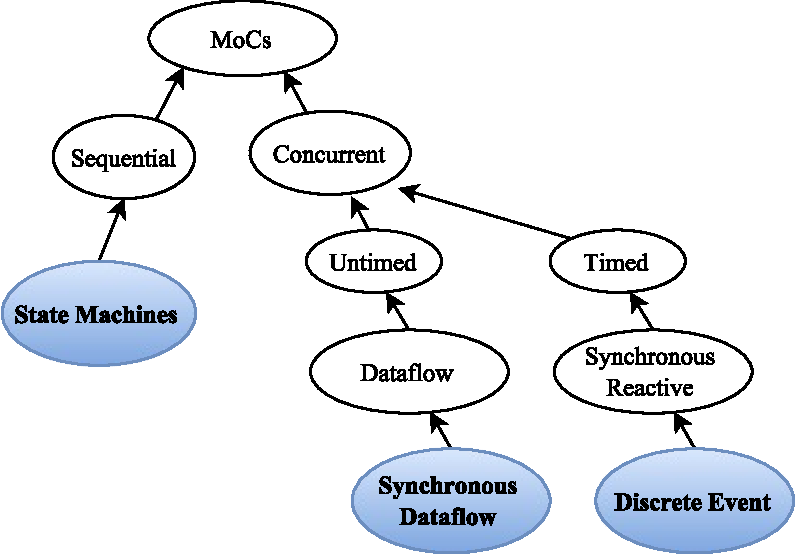
\includegraphics[width=.9\linewidth]{Figures/MoCs.pdf}
\caption{\label{fig:orgparagraph1}
Categorization of three of the most explored MoCs: State Machine, Synchronous Dataflow and Discrete Event(adopted from \cite{Editor2014})}
\end{figure}


\subsection{The Discrete Event Model of Computation}
\label{sec:orgheadline4}
The dominant MoC that underlies most industry standard EDA languages (VHDL, Verilog, SystemC) is called \textbf{Discrete Event (DE)}.
The components of a DE system are called \textbf{processes}.
In this context processes usually model the behavior and functionality of hardware entities.
The execution of processes is concurrent and the communication is achieved through \textbf{events}.
An event can be considered as an exchange of a time-stamped value.

Concurrent execution does not imply parallel/simultaneous execution. 
The notion of \textbf{concurrency} is more abstract. 
It can be realized as either parallel/simultaneous execution or as sequential interleaved execution, depending on the actual machine's computational resources.

Systems whose semantics are meant to be interpreted by a DE MoC, in order to be realizable, must have a \textbf{causal} behavior: they must process events in a chronological order, 
while any output events produced by a process are required to be no earlier in time than the input events that were consumed \cite{Editor2014}.
At any moment in real time, the model's time is determined by the last event processed.

In figure \ref{fig:orgparagraph1} one can observe that the DE MoC is also considered to be \textbf{Synchronous-Reactive (SR)}. 
This demonstrates the possibility of the MoC to "understand" entities with zero execution time, where output events are produced at the same time input events are consumed.
We can also extend/rephrase the previous definitions and say that Synchronous-Reactive MoCs are able to handle systems where events happen at the same time, instantaneously, in a causal way.
The DE MoC handles the aforementioned situations by extending time-stamps(the notion of model time) with the introduction of delta delays (also referred to as cycles or micro-steps).
A delta delay signifies an infinitesimal unit of time and no amount of delta delays, if summed, can result in time progression.
A time-stamp is therefore represented as a tuple of values, \((t,n)\) where \(t\) indicates the model time and \(n\) the number of delta delays that have advanced at \(t\).




\subsection{The Discrete Event Simulation(or)}
\label{sec:orgheadline5}
A realization of the DE abstract machine is called a \textbf{Discrete Event Simulator (DES)}.
SystemC's reference implementation of the DES is referred to as the \textbf{SystemC kernel} \cite{OpenSystemCInitiative2012}.

Concurrency of the system's processes is achieved through the co-routine mechanism (also known as co-operative multitasking). 
Processes execute without interruption. In a single core machine that means that only a single process can be running at any real time, 
and no other process instance can execute until the currently executing process instance has yielded control to the kernel.
A process shall not preempt or interrupt the execution of another process \cite{OpenSystemCInitiative2012}.

To avoid quantization errors and the non-uniform distribution of floating point values, time is expressed as an integer multiple of a real value referred to as the time resolution. 

The kernel maintains a \textbf{centralized event queue} that is sorted by time-stamp and knows which process is \textbf{running}, which processes are waiting for events and which are \textbf{runnable}.
Runnable processes have had events to which they are sensitive triggered and are waiting for the running process to yield to the kernel so that they can be scheduled.
The kernel controls the execution order by selecting the earliest event in the event queue and making its time-stamp the current simulation time.
It then determines the process the event is destined for, and finds all other events in the event queue with the same time-stamp that are destined for the same process \cite{Black2010}.
The operation of the kernel is exemplified in Alg \ref{alg:kernel}.

\begin{algorithm}
\caption{SystemC event loop, adopted from \cite{Schumacher2010}}
\label{alg:kernel}
\begin{algorithmic}[1]

   \While{timed events to process exist}  \Comment{Simulation time progression}
      \State trigger events at that time
      \While {runnable processes exist}   \Comment{Delta cycle progression}
         \While {runnable processes exist}
	     \State run all triggered processes
             \State trigger all immediate notifications
         \EndWhile
         \State update values of changed channels
	 \State trigger all delta time events
       \EndWhile
       \State advance time to next event time
   \EndWhile

\end{algorithmic}
\end{algorithm}


\subsection{The Parallel Discrete Event Simulation(or)}
\label{sec:orgheadline6}
The previous section has made evident that the reference implementation of the SystemC kernel assumes sequential execution and therefore can not utilize modern massively parallel host platforms. 
The most logical step in achieving faster simulations is to realize concurrency, from interleaving process execution to actual simultaneous/parallel execution.
By assigning each process to a different processing unit of the host platform (core or hardware thread) we enter the domain of \textbf{Parallel Discrete Event Simulation (PDES)}.
SystemC as a SLDL remains the same while the implementation of the DES is radically different.

By allowing processes to execute simultaneously one can allow each process to have its own perception of simulation time, determined by the last event it received.
This approach is referred to as \textbf{Out-of-Order PDES (OoO PDES)} \cite{Chen2015}.
Examples of OoO PDES simulators are the SystemC-SMP \cite{Mello2010} and SpecC \cite{Domer2011}, although the latter is not meant for SystemC.

For PDES implementations that enforce global simulation time, the term Synchronous PDES has been coined in the parSC simulator\cite{Schumacher2010}.
In Synchronous PDES, parallel execution of processes is performed within a delta cycle. 
With respect to Alg \ref{alg:kernel}, we can say that a Synchronous PDES parallelizes the execution of the innermost loop (line 4).
However, as we will see in the following section, this approach will bare no fruits in the simulation of TLM Loosely Timed simulations, since delta cycles are rarely triggered \cite{Chen2012}.

Finally, before committing into modifying the SystemC DES, we should mention the existence of less intrusive approaches, that instead of redesigning extend the reference kernel.
The example of the sc-during SystemC library \cite{Moy} is characteristic. 
To exploit parallelism, each process must be redefined as a sequence of atomic tasks that have duration (in simulation time).
The term atomic is used to represent the fact that these tasks are insensitive to input/output events for their duration.
Thus, the kernel can safely assign them to a different operating system thread and allow them to execute independently from the rest of the simulation.



\subsection{Transaction Level Modeling}
\label{sec:orgheadline7}
\textbf{Transaction Level Modeling (TLM)} enhances SystemC's expressiveness in order to facilitate the more abstract description (compared to RTL) of systems.  
TLM 2.0 allows model interoperability and the rapid development of fast virtual platforms to be deployed in software development, early on in the system's design procedure.

Transaction-level models represent one specific type of the DE MoC \cite{Grotker2002}.
Transactions are non-atomic communications, normally with bidirectional data transfer, and consist of a set of messages that are usually modeled as atomic communications.
The set of messages exchanged during a transaction are modeled using function calls and represent the different phases of a communication protocol.
In a transaction one can distinguish two actors:
the \textbf{initiator}, the process which initiated the communication, and the \textbf{target}, the process which is supposed to service the target's request.

TLM 2.0 API \cite{OpenSystemCInitiative2009} consists of the following features:
\begin{itemize}
\item A set of core interfaces
\begin{itemize}
\item A Blocking interface which is coupled with the \textbf{Loosely-Timed (LT)} coding style.
\item A non-blocking interface, which is coupled with the \textbf{Approximately-Timed (AT)} coding style.
\item The \textbf{Direct Memory Interface (DMI)} to enable an initiator to have direct access to a target's memory, bypassing the usual path through the interconnect components used by the transport interfaces.
\item The \textbf{Debug transport interface} to allow an non-intrusive inspection of the system's state.
\end{itemize}
\item The \textbf{global quantum} used by the \textbf{temporal decoupling} mechanism of the LT coding style, which facilitates faster simulations by reducing the number of context switches performed by the kernel.
\item Initiator and target \textbf{sockets} to denote the links (causal dependencies) between processes.
\item The \textbf{generic payload} which supports the abstract modeling of memory-mapped buses.
\item A set of \textbf{utilities} to facilitate the rapid development of models.
\end{itemize}

Figure demonstrates the typical use cases for TLM's different features.
\begin{figure}[htb]
\centering
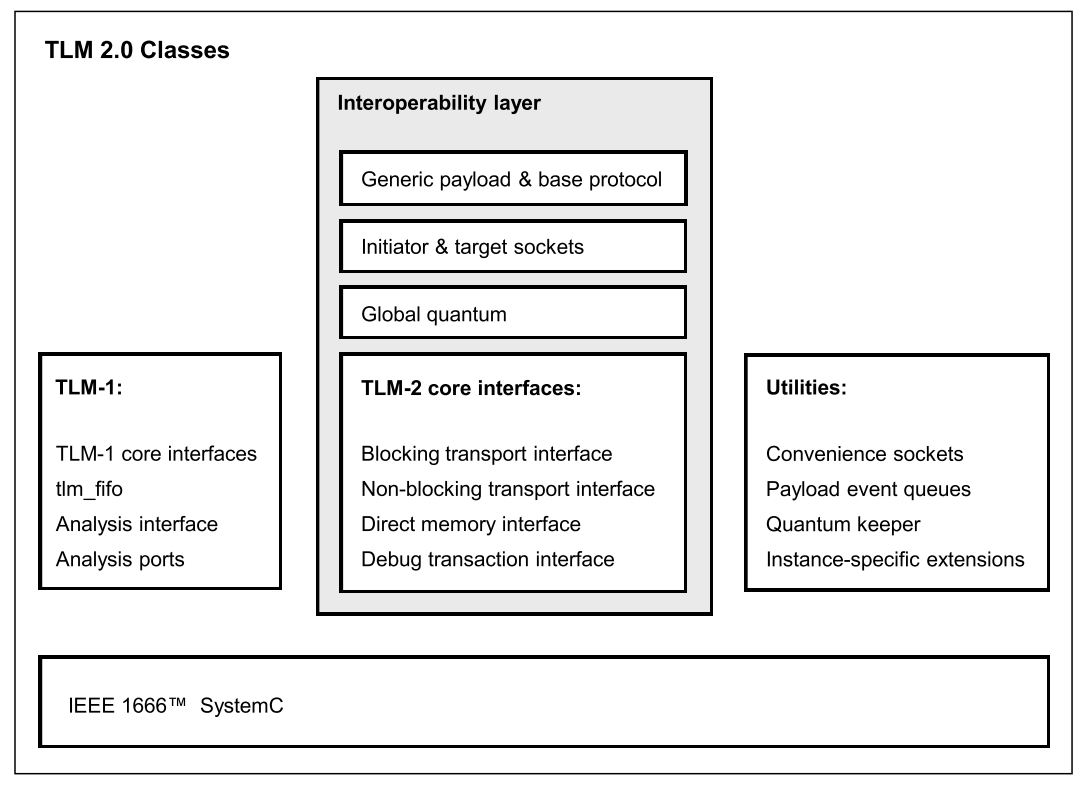
\includegraphics[width=.9\linewidth]{Figures/tlm_use_cases.png}
\caption{\label{fig:orgparagraph2}
TLM 2.0 use cases (adopted from \cite{OpenSystemCInitiative2009}).}
\end{figure}




\section{Problem statement}
\label{sec:orgheadline9}
The distribution of simulation time opens Pandora's box. 
Protecting the OoO PDES from \textbf{causality errors} demands certain assumptions and the addition of complex implementation mechanisms.

The first source of causality errors arises when the system's state variables are not distributed, in a disjoint way, among the processes \cite{Fujimoto1990}.
A trivial realization of the above scenario is depicted in figure \ref{fig:orgparagraph3}. Processes \(P_1\) and \(P_2\) are executing simultaneously, while sharing the system's state variable \(x\).
Events \(E_1\) and \(E_2\) are executed by \(P_1\) and \(P_2\) respectively. If we assume that in real time \(E_2\) is executed before \(E_1\), then we have implicitly broken causality, since \(E_1\) might be influenced
by the value of \(x\) that the execution of \(E_2\) might have modified. Furthermore, one must observe that this kind of implicit interaction between \(P_1\) and \(P_2\) can not be expressed in a DE MoC. 
This is a meta-implication of the host platform's shared memory architecture.

\begin{figure}[htb]
\centering
\includegraphics[width=.9\linewidth]{Figures/causality_shared_state.png}
\caption{\label{fig:orgparagraph3}
Causality error caused by the sharing of the system's state variable \(x\) by \(P_1\) and \(P_2\).}
\end{figure}

The second and most difficult to deal with source of causality errors is depicted in figure \ref{fig:orgparagraph4}. 
Event \(E_1\) affects \(E_2\) by scheduling a third event \(E_3\) which, for the shake of argument, modifies the state of \(P_2\). 
This scenario necessitates sequential execution of all three events. 
Thus the fundamental problem in PDES, in the context of this scenario, becomes the question: how can we deduce that it is safe to execute \(E_2\) in parallel with \(E_1\), without actually executing \(E_1\) \cite{Fujimoto1990}?
However, one must notice that the kind of interaction that yields this problematic situation is explicitly stated in the model.

\begin{figure}[htb]
\centering
\includegraphics[width=.9\linewidth]{Figures/causality_safe_events.png}
\caption{\label{fig:orgparagraph4}
Causality error caused by the unsafe execution of event \(E_2\) (adopted from \cite{Fujimoto1990}).}
\end{figure}

The last example makes evident the fact that the daunting task of preserving causality in the simulation is all about \textbf{process synchronization}.
For example, each process must be able to communicate to each of its peers (processes that is linked with) the message: 
"I will not send you any event before \(t_1\), so you can proceed with processing any event you have with time-stamp \(t_2\) where \(t_2 < t_1\)".

PDES synchronization algorithms, with respect to how they deal with causality errors, have been classified into two categories: \textbf{conservative} and \textbf{optimistic} \cite{Fujimoto2015}.
Conservative mechanisms strictly avoid the possibility of any causality error ever occurring by means of model introspection and static analysis.
On the other hand, optimistic/speculative approaches use a detection and recovery approach: when causality errors are detected a rollback mechanism is invoked to restore the system.
An optimistic compared to a conservative approach will theoretically yield better performance in models where communication, thus the probability of causality errors, is below a certain threshold \cite{Fujimoto1990}.

Both groups present severe implementation difficulties.
For conservative algorithms, model introspection and static analysis tools might be very difficult to develop,
while the rollback mechanism of an optimistic algorithm may require complex entities, such as a hardware/software transactional memory \cite{Anane2015} .


\section{Problem}
\label{sec:orgheadline10}
In this project we investigate the feasibility of implementing a SystemC OoO PDES, 
that can lead to scalable simulations of MPSoC Loosely-Timed Transaction Level Models,
on SMP host platforms.


\section{Hypothesis}
\label{sec:orgheadline11}
We hypothesize that by following a conservative approach on implementing a SystemC OoO PDES 
we will yield semantically equivalent and scalable simulations with respect to the reference SystemC DES.   


\section{Purpose}
\label{sec:orgheadline12}
The vision of a fully automated and connected society, the IoT revolution has promised to deliver,
is depending on the industry's ablate to deliver novel, complex and heterogeneous cyber-physical systems with short time-to-market constraints.
To live up to these expectations, the engineering discipline of ESLD must provide an answer to a number of questions:
\newline
\textbf{High-Level Synthesis}: How a system described in a SLDL can be realized in a structured and automatic way? 
Which of its components should be mapped in hardware entities like Digital Signal Processors (DSPs), Field Programmable Gate Arrays (FPGAs) or Application Specific Integrated Circuits (ASICs)?
Which of its components could be software for some kind of Central Processing Unit (CPU)?
Which is the optimal mapping that satisfies the system's requirements and yields a minimum power consumption?
\newline
\textbf{Correct-by-design}: Can a high-level synthesis design methodology yield correct-by-design implementations?
Can a system be formally verified given its abstract representation, early on in the design procedure?
Can we free the huge amount of resources wasted in mundane testing and debugging procedures that sometimes can not even provide any formal guarantee about the system's behavior?
\newline
\textbf{Improving the co-simulation speed for hardware and software}: Can we develop a virtual prototype of the platform early on in the development cycle, 
so that software engineers can begin developing integral applications without having to wait for the silicon to arrive?
Can we make the simulation fast and accurate, utilizing all the latest developments in High Performance Computing (HPC)?
This project hopes to deliver an infinitesimal contribution in solving the latter class of questions.





\section{Goals and Objectives}
\label{sec:orgheadline13}
If the timing constraints stretched beyond the scope of a Master Thesis, 
the project's self-actualization would require the development/production of the following components (sorted in descending significance order):
\begin{enumerate}
\item An OoO PDES implementation of the SystemC kernel.
\item A proof of concept application of the proposed kernel, on a sufficiently parallel system, running a substantially parallel application, on top of a Linux kernel.
\item The Master Thesis report document.
\item A static analysis/introspection tool for parsing the SystemC description of the system and extracting its pure representation, in terms of processes and links.
\item A code generation tool for constructing the communication and synchronization mechanisms.
\item A way of sequencing the application of the previous tools, either in the kernel's elaboration phase, or using a "gluing" script.
\item A TLM 2.0 coding style to minimize the effort and complexity of the analysis and generation tools.
\item A way to ensure the kernel's OSCI compliance.
\item A roadmap for elevating the simulation from SMP parallel to distributed, in a cluster of SMP nodes, parallel.
\end{enumerate}

Given the time constraints, the primary focus falls on the first three objectives.
The automation and generality the tools could deliver will be emulated by manual and ad-hoc solutions.







\section{Methods}
\label{sec:orgheadline19}
\subsection{Assumptions and delimitations}
\label{sec:orgheadline14}
The IEEE Standard for SystemC states the following about non reference implementations of the kernel:
"An implementation running on a machine that provides hardware support for concurrent processes may permit two or more processes to run concurrently
provided that the behavior appears identical to the co-routine semantics defined in this subclause.
In other words, the implementation would be obliged to analyze any dependencies between processes and to constrain their execution to match the co-routine semantics " \cite{OpenSystemCInitiative2012}.
We assume that our implementation, since it is designed to deliver causal simulations, has a strong coverage over this directive (consider the TLM 2.0 temporal decoupling technique which often yields inaccurate simulations)

However, the feasibility of the introspection and code generation procedures, imposes certain limitations on SystemC's expressive capabilities.
This is the main reason our kernel can not be considered to be compliant with the standard.

We also state that by assuming/enforcing the principle of one process per module and not allowing a module to execute another module's functions in its context (TLM 2.0 blocking transport interface), 
we hope to avoid causality errors caused by processes sharing system variables.




\subsection{Process synchronization algorithm}
\label{sec:orgheadline15}
We will begin our experimentations using a class of conservative synchronization algorithms originating from the work of \textbf{Chandy/Misra/Bryant (CMB)} \cite{Bryant,Chandy1979}.
Listing \ref{alg:kernel} demonstrates how these algorithms deal with the fundamental dilemma presented in section \ref{sec:orgheadline9}, figure \ref{fig:orgparagraph4}.

\begin{algorithm}
\caption{Process event loop, adopted from \cite{Fujimoto1999}}
\label{alg:initial_CMB}
\begin{algorithmic}[2]

   \While{simulation is not over}  
      \State \textbf{Block} until each incoming link queue contains at least one event
      \State remove event with the smallest time-stamp M from its queue.
      \State set clock = M
      \State process M
   \EndWhile

\end{algorithmic}
\end{algorithm}

However, a naive realization of the algorithm leads to deadlock situations like the one depicted in figure \ref{fig:orgparagraph5}.
The queues placed along the red loop are empty, thus simulation has halted, even though there are pending events (across the blue loop).

\begin{figure}[htb]
\centering
\includegraphics[width=.9\linewidth]{Figures/Deadlock.png}
\caption{\label{fig:orgparagraph5}
adopted from \cite{Fujimoto1999}}
\end{figure}

The deadlock avoidance mechanism that lies in the core of the CMB class of algorithms can be demonstrated with the following example:
Let us assume that \(P_3\) is at time 5.
Furthermore, let us assume that we have the \textbf{a priori} knowledge that \(P_3\) has a minimum event processing time of 3 (simulated).
We will call this knowledge \textbf{lookahead}.
\(P_3\) could create a \textbf{null event}, with no data value, but with a time-stamp \(t\)(8) = clock(5) + lookahead(3) and place it on its outgoing links.
A null event is still an event, so \(P_2\) by processing it would advance its clock to 8.
In the same fashion, let us assume that \(P_2\) has a lookahead of 2 and upon processing \(P_3\) null event, 
it will generate a null event for \(P_1\) with time-stamp 10. 
Eventually \(P_1\) can now safely process actual event with time-stamp 9, thus unfreezing the simulation.

The important points one must notice with this deadlock avoidance mechanism are that:
\begin{itemize}
\item Null events are created when a process updates its clock.
\item Each process propagates null events on all of its outgoing links.
\item This mechanism is mostly dependent to determine sufficiently large lookaheads.
\end{itemize}




\subsection{Introspection and code generation}
\label{sec:orgheadline16}
For the critical task of analyzing the model, identifying the processes and the links between them, we will follow ForSyDe SystemC's approach \cite{Hosein2012}.
Using SystemC's well defined API for module hierarchy (e.g. \texttt{get\_child\_objects()}), along with the introduction of meta objects, the system's structure can be
serialized at runtime, in the pre simulation phase of elaboration.




\subsection{Hardware and Software tools}
\label{sec:orgheadline17}
To ensure efficiency and code readability, we will use the explicit threading mechanisms that come with the latest standards of C++.
The Intel Parallel Studio XE 2016 toolchain will be used for compilation, code analysis and optimization.
We will initially use the Intel® Xeon Phi™ 5120D Coprocessor as the host platform for the simulation.
The coprocessor is situated in a Intel® Xeon E5-2600M v3 server (named lovisa).



\subsection{Evaluation Metrics}
\label{sec:orgheadline18}
The first evaluation metric of the proposed kernel will be its strong scalability against the reference SystemC kernel.
It will be determined by keeping the simulation's size constant and varying the number of processing elements.
Furthermore, we will also measure weak scalability, by varying the number of processing elements and the simulation's size symmetrically,
and trying to achieve constant time to simulation end.

The simulation's size can be easily related to the duration of the simulation (in simulated time).
Another way of describing the simulation's size is through the conception of a formula involving the number of system processes, the number of links, the system's topology and the amount of events generated.

The accuracy of the simulation can be measured by the aggregate number of causality errors.
The detection of causality errors must be facilitated in a per process level and the aggregation shall be performed at the end of the simulation.
A concrete realization of the accuracy metric comes in the form of a counter each process increments whenever it executes an event with a time-stamp lower than its clock (the time-stamp of the last processed event).



\section{Tasks and Time Scheduling}
\label{sec:orgheadline20}
The majority of the remaining time has been partitioned into 3 x 3-4 week long iterations, 
where we will incrementally try to achieve our objectives.
The tasks that comprise the first iteration are the following:
\begin{enumerate}
\item Setup software environment on the first experimentation server (Lovisa)
\item Manually compile the TLM 2.0 LT example of the SystemC installation, to a multithreaded C++ application, according to the CMB algorithm.
\item Document Task 1
\item Find a way to create parameterizable random networks within C++, that can be serialized in a form Matlab can analyze and visualize them.
\item Create "dummy" process functionality that resembles the behavior of common TLM actors (Instruction Set Simulators, Memory, Timers etc)
\item Perform a number of simulations of the random systems that correspond to the random networks.
\item Document Tasks 3-5.
\end{enumerate}

The context of the next iterations will be decided based on the outcome of the first.
To summarize:

\begin{center}
\begin{tabular}{rrrl}
\textbf{Week(s)} & \textbf{End Date} & \textbf{Task Number} & \textbf{Milestone}\\
\hline
5-7 & 02-18 & Initial Investigation & Project Plan v1\\
\hline
7 & 02-19 & 1 & \\
\hline
8 & 02-26 & 2 & \\
\hline
9 & 03-02 & 3 & Status Report 1\\
\hline
9 & 03-04 & 4 & \\
\hline
10 & 03-11 & 5 & \\
\hline
11 & 03-18 & 6 & \\
\hline
12 & 03-23 & 7 & Status Report 2\\
\hline
12-15 & 04-14 & Second Iteration & Status Report 3\\
\hline
16-19 & 05-12 & Third  Iteration & Status Report 4\\
\hline
20-21 &  & Reserve weeks & \\
\hline
22-26 & 06-30 & Project closure & Final Report\\
\end{tabular}
\end{center}


\section{References}
\label{sec:orgheadline21}
\renewcommand\refname{}
\bibliography{References}
\bibliographystyle{myIEEEtran}
\end{document}
